\section{Preliminaries on curved folding} \label{sec:pre}
In the following we summarize common knowledge on curved folding, relevant for our work. By a curved folded surface we mean a piecewise $C^2$ developable surfaces, whose discontinuities are focused along creases. We assume that these creases are $C^2$ curves that may intersect one another, and we call these intesection points \textit{vertices}. These curves segment the surface into various disconnected components, which we call curved patches. By our assumptions these curved patches remain $C^2$, i.e. though the folding operation creates discontinuities along patches, the patches viewed separately are deformed by $C^2$ deformations. Throughout the paper we will often visualize the crease pattern itself, i.e. the initial flatten surface together with its curved creases (\figref{crease_pattern}).

\begin{figure} [h]
	\centering
	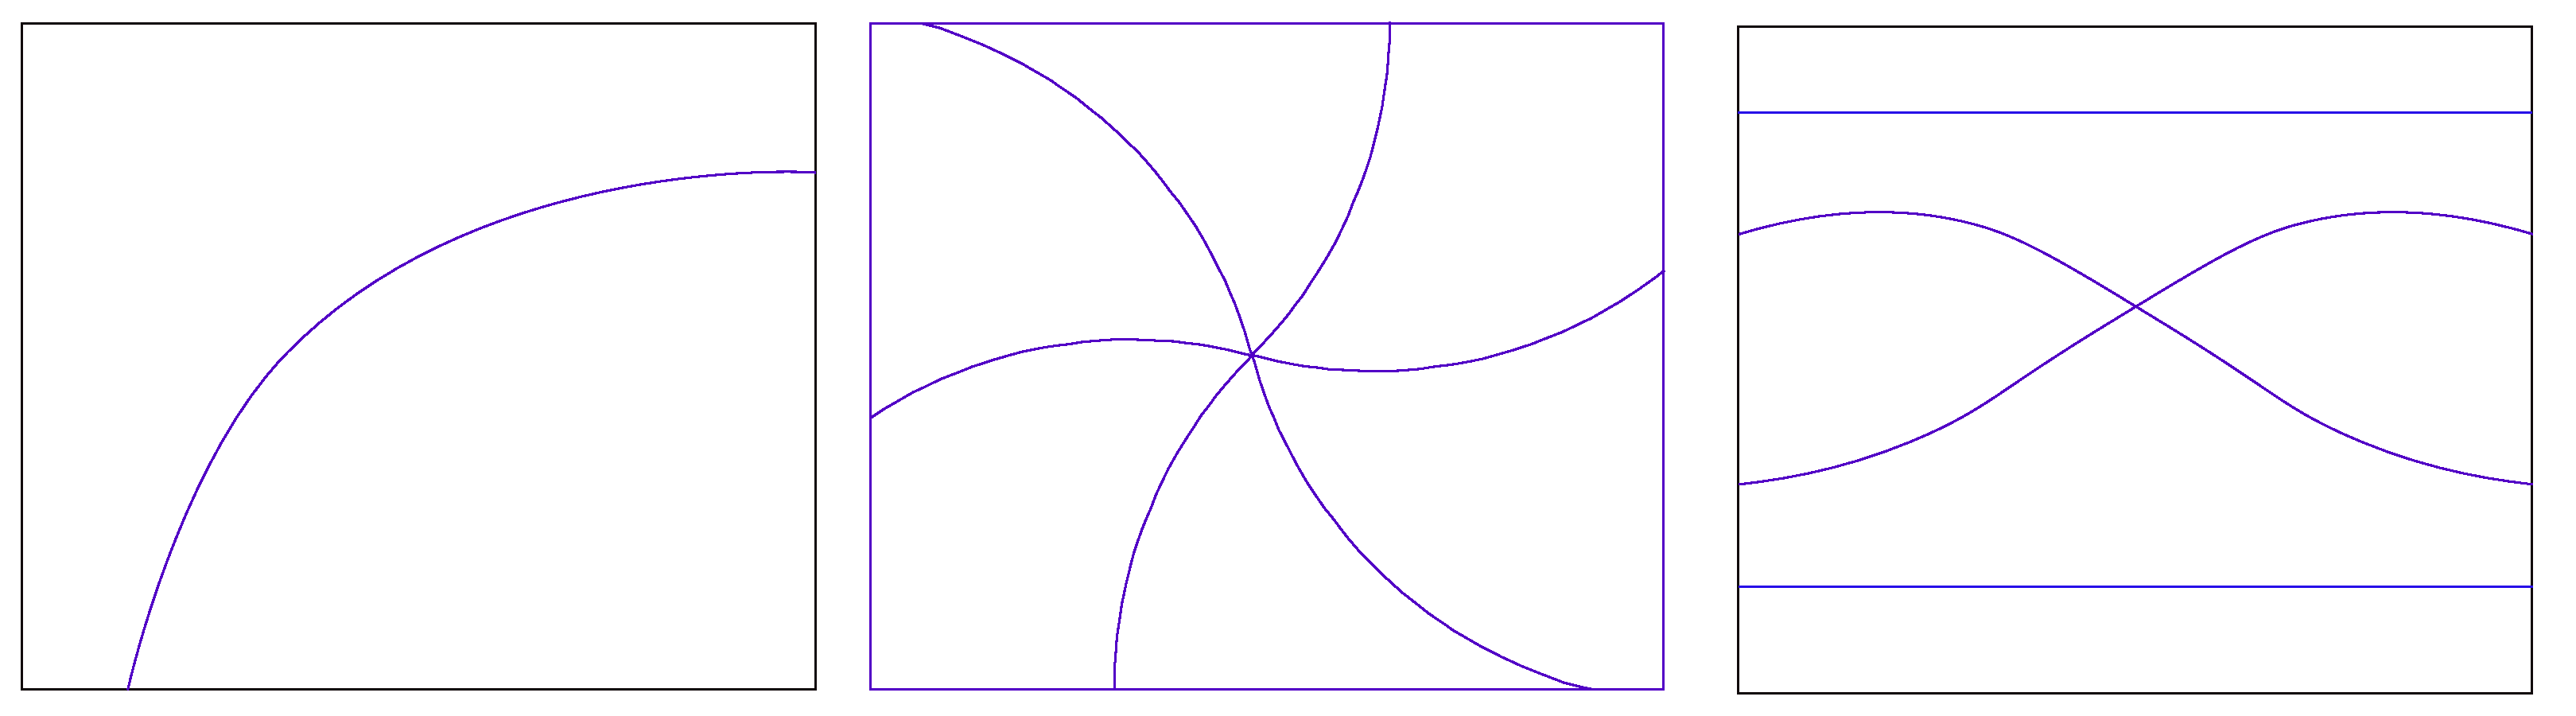
\includegraphics[width=\linewidth]{figures/crease_patterns}
	\caption{Creased patterns.}
	\label{fig:crease_pattern}
\end{figure}

\subsection{Curved folding from the view of a curve} \label{sec:curved_folding_from_a_curve}
Let $\Gamma(t)$ be a curve on a smooth developable surface $S$,  let $\gamma(t)$ be its flattened curve, $k(t)$ its curvature, and $k_g(t)$ its geodesic curvature such that $k_g(t) = k(t) \cos(\alpha(t))$ for some $\alpha \neq 0$. This implies that at each point along $\Gamma(t)$, the tangent planes of $S$ make an angle of $\alpha$ with the osculating planes of $\Gamma(t)$. One can switch this point of view: start with a flat curve $\gamma(t)$, isometrically embed the curve in $\mathbb{R}^3$ and construct a developable surface by reconstructing the planes at each point. As long as the crease is curved, i.e. has some normal curvature such that $k(t) > k_g(t)$ and $\alpha(t) \neq 0$ then there are 2 distinct planes containing $\Gamma'(t)$ and forming an angle of $\alpha(t)$ with the curve's osculating plane. Therefore, one can locally construct two different smooth developable surfaces passing through $\Gamma(t)$ with $\gamma(t)$ as its flattening. Alternatively, one can construct a folded surface by a consistent smooth choice of a different tangent plane for each "side" of the curve (see Fig. \ref{fig:curved_fold_through_curve}) \cite{more_on_paper}.

\begin{figure} [h]
	\centering
	\includegraphics[width=0.7\linewidth]{figures/curved_fold_through_curve.pdf}
	\caption{(TODO BETTER FIG) Left: A flattened curve in 2D. Right: A small neighbourhood around an embedding of the curve in $\mathbb{R}^3$, its osculating plane and two options to extend a the curve to developable surface by constructing the 2 planes containing the curve's tangent and making an angle of $\alpha(t)$  with the osculating plane. Choosing 2 different tangents along each 'side' of the curve creates discontinuities along the curve and a curved folded surface.}
	\label{fig:curved_fold_through_curve}
\end{figure}

%Two intersecting developable surfaces can be flattened along their intersection if the intersected curve have the same geodesic curvature on both surfaces. 
\subsection{Number of ways to fold a single curved crease}
A single straight crease is rather boring, mathematically speaking. Straight lines can only be folded as in classical origami, i.e. by keeping them straight \cite{demaine_lens}. Hence the folding process of a single fold can be described by a single real number, representing the fold dihedral angle. The results at section \secref{sec:curved_folding_from_a_curve} however showed that there are far more degrees of freedom for folding a curved crease; Up to rigid motion, this folding could be described by two smooth \textit{functions}: the curves' curvature $k(t) \geq k_g(t)$ and its torsion $\tau(t)$. Unlike the case of classical origami, the folding angle of a curved crease can vary along the curve. The curvature and torsion also dictates the ruling patterns of the developable surfaces, generally changing while folding and bending the surface. %(there's the cone singularity case where a curved fold is more local (as focused on the cone point) but I think this requires the curve to be C^1.. should mention it?

\subsection{Multiple creases}
Deforming a curved crease locally determines the shape of both surfaces around it, unlike the case of a straight fold. If a folded surfaces consists of more than 2 patches then this deformation further propagates, as seen in fig ADD-FIG. The propagation depends on the rulings direction, though as mentioned these can smoothly change during the deformation itself.
% Say how one crease set the entire shapes, and how this propagates. Say that at that point there is a binary choice, fold or not fold. Hence once you choose M/V assignment (choice of surface), you can often locally just choose bla bla. We don't know how to handle more general cases, vertices, stars, etc.
%This is a more limited operation, as one can only assign a single folding angle as opposed to two real valued smooth functions, however folding along a straight line doesn't fix the shape of the surrounding surface as in the case of a curved crease.
